% Options for packages loaded elsewhere
\PassOptionsToPackage{unicode}{hyperref}
\PassOptionsToPackage{hyphens}{url}
\PassOptionsToPackage{dvipsnames,svgnames,x11names}{xcolor}
%
\documentclass[
]{article}
\usepackage{amsmath,amssymb}
\usepackage{iftex}
\ifPDFTeX
  \usepackage[T1]{fontenc}
  \usepackage[utf8]{inputenc}
  \usepackage{textcomp} % provide euro and other symbols
\else % if luatex or xetex
  \usepackage{unicode-math} % this also loads fontspec
  \defaultfontfeatures{Scale=MatchLowercase}
  \defaultfontfeatures[\rmfamily]{Ligatures=TeX,Scale=1}
\fi
\usepackage{lmodern}
\ifPDFTeX\else
  % xetex/luatex font selection
\fi
% Use upquote if available, for straight quotes in verbatim environments
\IfFileExists{upquote.sty}{\usepackage{upquote}}{}
\IfFileExists{microtype.sty}{% use microtype if available
  \usepackage[]{microtype}
  \UseMicrotypeSet[protrusion]{basicmath} % disable protrusion for tt fonts
}{}
\makeatletter
\@ifundefined{KOMAClassName}{% if non-KOMA class
  \IfFileExists{parskip.sty}{%
    \usepackage{parskip}
  }{% else
    \setlength{\parindent}{0pt}
    \setlength{\parskip}{6pt plus 2pt minus 1pt}}
}{% if KOMA class
  \KOMAoptions{parskip=half}}
\makeatother
\usepackage{xcolor}
\usepackage[margin=1in]{geometry}
\usepackage{color}
\usepackage{fancyvrb}
\newcommand{\VerbBar}{|}
\newcommand{\VERB}{\Verb[commandchars=\\\{\}]}
\DefineVerbatimEnvironment{Highlighting}{Verbatim}{commandchars=\\\{\}}
% Add ',fontsize=\small' for more characters per line
\usepackage{framed}
\definecolor{shadecolor}{RGB}{248,248,248}
\newenvironment{Shaded}{\begin{snugshade}}{\end{snugshade}}
\newcommand{\AlertTok}[1]{\textcolor[rgb]{0.94,0.16,0.16}{#1}}
\newcommand{\AnnotationTok}[1]{\textcolor[rgb]{0.56,0.35,0.01}{\textbf{\textit{#1}}}}
\newcommand{\AttributeTok}[1]{\textcolor[rgb]{0.13,0.29,0.53}{#1}}
\newcommand{\BaseNTok}[1]{\textcolor[rgb]{0.00,0.00,0.81}{#1}}
\newcommand{\BuiltInTok}[1]{#1}
\newcommand{\CharTok}[1]{\textcolor[rgb]{0.31,0.60,0.02}{#1}}
\newcommand{\CommentTok}[1]{\textcolor[rgb]{0.56,0.35,0.01}{\textit{#1}}}
\newcommand{\CommentVarTok}[1]{\textcolor[rgb]{0.56,0.35,0.01}{\textbf{\textit{#1}}}}
\newcommand{\ConstantTok}[1]{\textcolor[rgb]{0.56,0.35,0.01}{#1}}
\newcommand{\ControlFlowTok}[1]{\textcolor[rgb]{0.13,0.29,0.53}{\textbf{#1}}}
\newcommand{\DataTypeTok}[1]{\textcolor[rgb]{0.13,0.29,0.53}{#1}}
\newcommand{\DecValTok}[1]{\textcolor[rgb]{0.00,0.00,0.81}{#1}}
\newcommand{\DocumentationTok}[1]{\textcolor[rgb]{0.56,0.35,0.01}{\textbf{\textit{#1}}}}
\newcommand{\ErrorTok}[1]{\textcolor[rgb]{0.64,0.00,0.00}{\textbf{#1}}}
\newcommand{\ExtensionTok}[1]{#1}
\newcommand{\FloatTok}[1]{\textcolor[rgb]{0.00,0.00,0.81}{#1}}
\newcommand{\FunctionTok}[1]{\textcolor[rgb]{0.13,0.29,0.53}{\textbf{#1}}}
\newcommand{\ImportTok}[1]{#1}
\newcommand{\InformationTok}[1]{\textcolor[rgb]{0.56,0.35,0.01}{\textbf{\textit{#1}}}}
\newcommand{\KeywordTok}[1]{\textcolor[rgb]{0.13,0.29,0.53}{\textbf{#1}}}
\newcommand{\NormalTok}[1]{#1}
\newcommand{\OperatorTok}[1]{\textcolor[rgb]{0.81,0.36,0.00}{\textbf{#1}}}
\newcommand{\OtherTok}[1]{\textcolor[rgb]{0.56,0.35,0.01}{#1}}
\newcommand{\PreprocessorTok}[1]{\textcolor[rgb]{0.56,0.35,0.01}{\textit{#1}}}
\newcommand{\RegionMarkerTok}[1]{#1}
\newcommand{\SpecialCharTok}[1]{\textcolor[rgb]{0.81,0.36,0.00}{\textbf{#1}}}
\newcommand{\SpecialStringTok}[1]{\textcolor[rgb]{0.31,0.60,0.02}{#1}}
\newcommand{\StringTok}[1]{\textcolor[rgb]{0.31,0.60,0.02}{#1}}
\newcommand{\VariableTok}[1]{\textcolor[rgb]{0.00,0.00,0.00}{#1}}
\newcommand{\VerbatimStringTok}[1]{\textcolor[rgb]{0.31,0.60,0.02}{#1}}
\newcommand{\WarningTok}[1]{\textcolor[rgb]{0.56,0.35,0.01}{\textbf{\textit{#1}}}}
\usepackage{graphicx}
\makeatletter
\def\maxwidth{\ifdim\Gin@nat@width>\linewidth\linewidth\else\Gin@nat@width\fi}
\def\maxheight{\ifdim\Gin@nat@height>\textheight\textheight\else\Gin@nat@height\fi}
\makeatother
% Scale images if necessary, so that they will not overflow the page
% margins by default, and it is still possible to overwrite the defaults
% using explicit options in \includegraphics[width, height, ...]{}
\setkeys{Gin}{width=\maxwidth,height=\maxheight,keepaspectratio}
% Set default figure placement to htbp
\makeatletter
\def\fps@figure{htbp}
\makeatother
\setlength{\emergencystretch}{3em} % prevent overfull lines
\providecommand{\tightlist}{%
  \setlength{\itemsep}{0pt}\setlength{\parskip}{0pt}}
\setcounter{secnumdepth}{5}
\usepackage[french]{babel}
\ifLuaTeX
  \usepackage{selnolig}  % disable illegal ligatures
\fi
\usepackage{bookmark}
\IfFileExists{xurl.sty}{\usepackage{xurl}}{} % add URL line breaks if available
\urlstyle{same}
\hypersetup{
  pdfauthor={Vincent Runge},
  colorlinks=true,
  linkcolor={Maroon},
  filecolor={Maroon},
  citecolor={Blue},
  urlcolor={blue},
  pdfcreator={LaTeX via pandoc}}

\title{Analyse des algorithmes de tri\\

\includegraphics[width=1in,height=\textheight]{Images/logo_lamme.png}

\includegraphics[width=1.7in,height=\textheight]{Images/logo_UEVE.png}\\
\strut ~M2 Data Science Algorithmique}
\author{Vincent Runge}
\date{lundi 147mars 2025}

\begin{document}
\maketitle

{
\hypersetup{linkcolor=}
\setcounter{tocdepth}{2}
\tableofcontents
}
\noindent\hrulefill

\section{Description du problème et
objectif}\label{description-du-probluxe8me-et-objectif}

Insertion sort is of time complexity \textbf{\(O(n^2)\)} as heap sort is
\textbf{\(O(n\log(n))\)} (worst case complexity). We aim at highlighting
two important features with this package:

\begin{enumerate}
\def\labelenumi{\arabic{enumi}.}
\tightlist
\item
  Rcpp algorithms are \textbf{much more efficient} than their R
  counterpart
\item
  Time complexities \textbf{can be compared to} one another
\end{enumerate}

\emph{All the simulations presented in this README file are available in
the \texttt{myTests.R} file in the forStudents folder which also
contains the Rmd file generating this README.md.}

Details on the heapsort algorithm can be found on
\href{https://en.wikipedia.org/wiki/Heapsort}{its wikipedia page}. This
gif provides a graphical representation of its mechanisms.

\subsubsection{Package installation}\label{package-installation}

You first need to install the \texttt{devtools} package, it can be done
easily from Rstudio. We install the package from Github (remove the \#
sign):

\begin{Shaded}
\begin{Highlighting}[]
\CommentTok{\#devtools::install\_github("vrunge/M2algorithmique")}
\FunctionTok{library}\NormalTok{(M2algorithmique)}
\end{Highlighting}
\end{Shaded}

\subsubsection{A first simple test}\label{a-first-simple-test}

We simulate simple data as follows, with \texttt{v} a vector as size
\texttt{n} containing all the integers from \texttt{1} to \texttt{n}
(exactly one time) in any order.

\begin{Shaded}
\begin{Highlighting}[]
\NormalTok{n }\OtherTok{\textless{}{-}} \DecValTok{10}
\NormalTok{v }\OtherTok{\textless{}{-}} \FunctionTok{sample}\NormalTok{(n)}
\end{Highlighting}
\end{Shaded}

We've implemeted 4 algorithms:

\begin{itemize}
\tightlist
\item
  \texttt{insertion\_sort}
\item
  \texttt{heap\_sort}
\item
  \texttt{insertion\_sort\_Rcpp}
\item
  \texttt{heap\_sort\_Rcpp}
\end{itemize}

They all have a unique argument: the unsorted vector \texttt{v}.

\begin{Shaded}
\begin{Highlighting}[]
\NormalTok{v}
\end{Highlighting}
\end{Shaded}

\begin{verbatim}
##  [1]  4  1  5  6  8  2  9  3  7 10
\end{verbatim}

\begin{Shaded}
\begin{Highlighting}[]
\FunctionTok{insertion\_sort}\NormalTok{(v)}
\end{Highlighting}
\end{Shaded}

\begin{verbatim}
##  [1]  1  2  3  4  5  6  7  8  9 10
\end{verbatim}

\texttt{insertion\_sort(v)} returns the sorted vector from \texttt{v}.

\subsection{The 4 algorithms at fixed data
length}\label{the-4-algorithms-at-fixed-data-length}

We run all the following examples at fixed vector length
\texttt{n\ =\ 10000}.

\subsubsection{One simulation}\label{one-simulation}

We define a function \texttt{one.simu} to simplify the simulation study
for time complexity.

\begin{Shaded}
\begin{Highlighting}[]
\NormalTok{one.simu }\OtherTok{\textless{}{-}} \ControlFlowTok{function}\NormalTok{(n, }\AttributeTok{type =} \StringTok{"sample"}\NormalTok{, }\AttributeTok{func =} \StringTok{"insertion\_sort"}\NormalTok{)}
\NormalTok{\{}
  \ControlFlowTok{if}\NormalTok{(type }\SpecialCharTok{==} \StringTok{"sample"}\NormalTok{)\{v }\OtherTok{\textless{}{-}} \FunctionTok{sample}\NormalTok{(n)\}}\ControlFlowTok{else}\NormalTok{\{v }\OtherTok{\textless{}{-}}\NormalTok{ n}\SpecialCharTok{:}\DecValTok{1}\NormalTok{\}}
  \ControlFlowTok{if}\NormalTok{(func }\SpecialCharTok{==} \StringTok{"insertion\_sort"}\NormalTok{)\{t }\OtherTok{\textless{}{-}} \FunctionTok{system.time}\NormalTok{(}\FunctionTok{insertion\_sort}\NormalTok{(v))[[}\DecValTok{1}\NormalTok{]]\}}
  \ControlFlowTok{if}\NormalTok{(func }\SpecialCharTok{==} \StringTok{"heap\_sort"}\NormalTok{)\{t }\OtherTok{\textless{}{-}} \FunctionTok{system.time}\NormalTok{(}\FunctionTok{heap\_sort}\NormalTok{(v))[[}\DecValTok{1}\NormalTok{]]\} }
  \ControlFlowTok{if}\NormalTok{(func }\SpecialCharTok{==} \StringTok{"insertion\_sort\_Rcpp"}\NormalTok{)\{t }\OtherTok{\textless{}{-}} \FunctionTok{system.time}\NormalTok{(}\FunctionTok{insertion\_sort\_Rcpp}\NormalTok{(v))[[}\DecValTok{1}\NormalTok{]]\}}
  \ControlFlowTok{if}\NormalTok{(func }\SpecialCharTok{==} \StringTok{"heap\_sort\_Rcpp"}\NormalTok{)\{t }\OtherTok{\textless{}{-}} \FunctionTok{system.time}\NormalTok{(}\FunctionTok{heap\_sort\_Rcpp}\NormalTok{(v))[[}\DecValTok{1}\NormalTok{]]\}}
  \FunctionTok{return}\NormalTok{(t)}
\NormalTok{\}}
\end{Highlighting}
\end{Shaded}

We evaluate the time with a given \texttt{n} over the 4 algorithms. We
choose

\begin{Shaded}
\begin{Highlighting}[]
\NormalTok{n }\OtherTok{\textless{}{-}} \DecValTok{10000}
\end{Highlighting}
\end{Shaded}

and we get:

\begin{Shaded}
\begin{Highlighting}[]
\FunctionTok{one.simu}\NormalTok{(n, }\AttributeTok{func =} \StringTok{"insertion\_sort"}\NormalTok{)}
\end{Highlighting}
\end{Shaded}

\begin{verbatim}
## [1] 1.814
\end{verbatim}

\begin{Shaded}
\begin{Highlighting}[]
\FunctionTok{one.simu}\NormalTok{(n, }\AttributeTok{func =} \StringTok{"heap\_sort"}\NormalTok{)}
\end{Highlighting}
\end{Shaded}

\begin{verbatim}
## [1] 0.578
\end{verbatim}

\begin{Shaded}
\begin{Highlighting}[]
\FunctionTok{one.simu}\NormalTok{(n, }\AttributeTok{func =} \StringTok{"insertion\_sort\_Rcpp"}\NormalTok{)}
\end{Highlighting}
\end{Shaded}

\begin{verbatim}
## [1] 0.009
\end{verbatim}

\begin{Shaded}
\begin{Highlighting}[]
\FunctionTok{one.simu}\NormalTok{(n, }\AttributeTok{func =} \StringTok{"heap\_sort\_Rcpp"}\NormalTok{)}
\end{Highlighting}
\end{Shaded}

\begin{verbatim}
## [1] 0.001
\end{verbatim}

\subsubsection{Some comparisons}\label{some-comparisons}

we compare the running time with repeated executions (\texttt{nbSimus}
times)

\begin{Shaded}
\begin{Highlighting}[]
\NormalTok{nbSimus }\OtherTok{\textless{}{-}} \DecValTok{10}
\NormalTok{time1 }\OtherTok{\textless{}{-}} \DecValTok{0}\NormalTok{; time2 }\OtherTok{\textless{}{-}} \DecValTok{0}\NormalTok{; time3 }\OtherTok{\textless{}{-}} \DecValTok{0}\NormalTok{; time4 }\OtherTok{\textless{}{-}} \DecValTok{0}

\ControlFlowTok{for}\NormalTok{(i }\ControlFlowTok{in} \DecValTok{1}\SpecialCharTok{:}\NormalTok{nbSimus)\{time1 }\OtherTok{\textless{}{-}}\NormalTok{ time1 }\SpecialCharTok{+} \FunctionTok{one.simu}\NormalTok{(n, }\AttributeTok{func =} \StringTok{"insertion\_sort"}\NormalTok{)\}}
\ControlFlowTok{for}\NormalTok{(i }\ControlFlowTok{in} \DecValTok{1}\SpecialCharTok{:}\NormalTok{nbSimus)\{time2 }\OtherTok{\textless{}{-}}\NormalTok{ time2 }\SpecialCharTok{+} \FunctionTok{one.simu}\NormalTok{(n, }\AttributeTok{func =} \StringTok{"heap\_sort"}\NormalTok{)\}}
\ControlFlowTok{for}\NormalTok{(i }\ControlFlowTok{in} \DecValTok{1}\SpecialCharTok{:}\NormalTok{nbSimus)\{time3 }\OtherTok{\textless{}{-}}\NormalTok{ time3 }\SpecialCharTok{+} \FunctionTok{one.simu}\NormalTok{(n, }\AttributeTok{func =} \StringTok{"insertion\_sort\_Rcpp"}\NormalTok{)\}}
\ControlFlowTok{for}\NormalTok{(i }\ControlFlowTok{in} \DecValTok{1}\SpecialCharTok{:}\NormalTok{nbSimus)\{time4 }\OtherTok{\textless{}{-}}\NormalTok{ time4 }\SpecialCharTok{+} \FunctionTok{one.simu}\NormalTok{(n, }\AttributeTok{func =} \StringTok{"heap\_sort\_Rcpp"}\NormalTok{)\}}
\end{Highlighting}
\end{Shaded}

\textbf{Rcpp is 100 to 200 times faster than R for our 2 algorithms.}

\begin{Shaded}
\begin{Highlighting}[]
\CommentTok{\#gain R {-}\textgreater{} Rcpp}
\NormalTok{time1}\SpecialCharTok{/}\NormalTok{time3}
\end{Highlighting}
\end{Shaded}

\begin{verbatim}
## [1] 205.191
\end{verbatim}

\begin{Shaded}
\begin{Highlighting}[]
\NormalTok{time2}\SpecialCharTok{/}\NormalTok{time4}
\end{Highlighting}
\end{Shaded}

\begin{verbatim}
## [1] 591.8889
\end{verbatim}

\textbf{With the data length of \texttt{10000}, heap\_sort runs 10 to 20
times faster than insert\_sort.}

\begin{Shaded}
\begin{Highlighting}[]
\CommentTok{\#gain insertion {-}\textgreater{} heap}
\NormalTok{time1}\SpecialCharTok{/}\NormalTok{time2}
\end{Highlighting}
\end{Shaded}

\begin{verbatim}
## [1] 3.428196
\end{verbatim}

\begin{Shaded}
\begin{Highlighting}[]
\NormalTok{time3}\SpecialCharTok{/}\NormalTok{time4}
\end{Highlighting}
\end{Shaded}

\begin{verbatim}
## [1] 9.888889
\end{verbatim}

\textbf{The gain between the slow insertsort R algorithm and the faster
heapsort Rcpp algorithm is of order 2000 !!!}

\begin{Shaded}
\begin{Highlighting}[]
\CommentTok{\#max gain}
\NormalTok{time1}\SpecialCharTok{/}\NormalTok{time4}
\end{Highlighting}
\end{Shaded}

\begin{verbatim}
## [1] 2029.111
\end{verbatim}

\subsection{Microblenchmark}\label{microblenchmark}

You need the packages \texttt{microbenchmark} and \texttt{ggplot2} to
run the simulations and plot the results (in violin plots). We compare
\texttt{insertion\_sort\_Rcpp} with \texttt{heap\_sort\_Rcpp} for data
lengths \texttt{n\ =\ 1000} and \texttt{n\ =\ 10000}.

\begin{Shaded}
\begin{Highlighting}[]
\FunctionTok{library}\NormalTok{(microbenchmark)}
\FunctionTok{library}\NormalTok{(ggplot2)}
\NormalTok{n }\OtherTok{\textless{}{-}} \DecValTok{1000}
\NormalTok{res }\OtherTok{\textless{}{-}} \FunctionTok{microbenchmark}\NormalTok{(}\FunctionTok{one.simu}\NormalTok{(n, }\AttributeTok{func =} \StringTok{"insertion\_sort\_Rcpp"}\NormalTok{), }\FunctionTok{one.simu}\NormalTok{(n, }\AttributeTok{func =} \StringTok{"heap\_sort\_Rcpp"}\NormalTok{), }\AttributeTok{times =} \DecValTok{50}\NormalTok{)}
\end{Highlighting}
\end{Shaded}

\begin{verbatim}
## Warning in microbenchmark(one.simu(n, func = "insertion_sort_Rcpp"),
## one.simu(n, : less accurate nanosecond times to avoid potential integer
## overflows
\end{verbatim}

\begin{Shaded}
\begin{Highlighting}[]
\FunctionTok{autoplot}\NormalTok{(res)}
\end{Highlighting}
\end{Shaded}

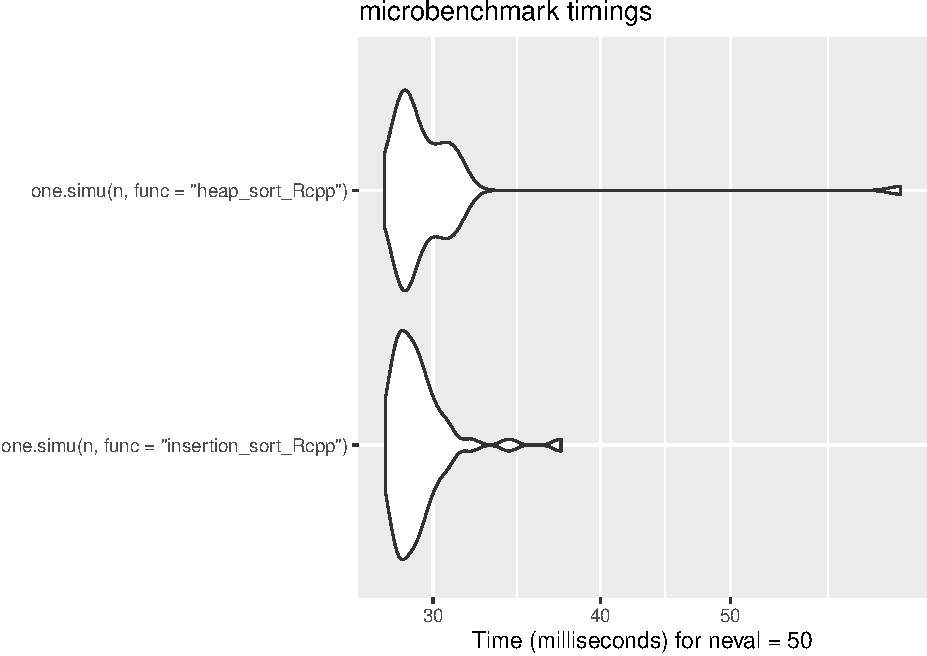
\includegraphics{Sorting_analyse_files/figure-latex/unnamed-chunk-11-1.pdf}

\begin{Shaded}
\begin{Highlighting}[]
\NormalTok{res}
\end{Highlighting}
\end{Shaded}

\begin{verbatim}
## Unit: milliseconds
##                                       expr      min       lq     mean   median
##  one.simu(n, func = "insertion_sort_Rcpp") 27.66426 28.35995 29.26405 28.92251
##       one.simu(n, func = "heap_sort_Rcpp") 27.59833 28.50381 30.06691 28.81324
##        uq      max neval
##  29.63193 37.37367    50
##  30.45259 66.95878    50
\end{verbatim}

\begin{Shaded}
\begin{Highlighting}[]
\NormalTok{n }\OtherTok{\textless{}{-}} \DecValTok{10000}
\NormalTok{res }\OtherTok{\textless{}{-}} \FunctionTok{microbenchmark}\NormalTok{(}\FunctionTok{one.simu}\NormalTok{(n, }\AttributeTok{func =} \StringTok{"insertion\_sort\_Rcpp"}\NormalTok{), }\FunctionTok{one.simu}\NormalTok{(n, }\AttributeTok{func =} \StringTok{"heap\_sort\_Rcpp"}\NormalTok{), }\AttributeTok{times =} \DecValTok{50}\NormalTok{)}
\FunctionTok{autoplot}\NormalTok{(res)}
\end{Highlighting}
\end{Shaded}

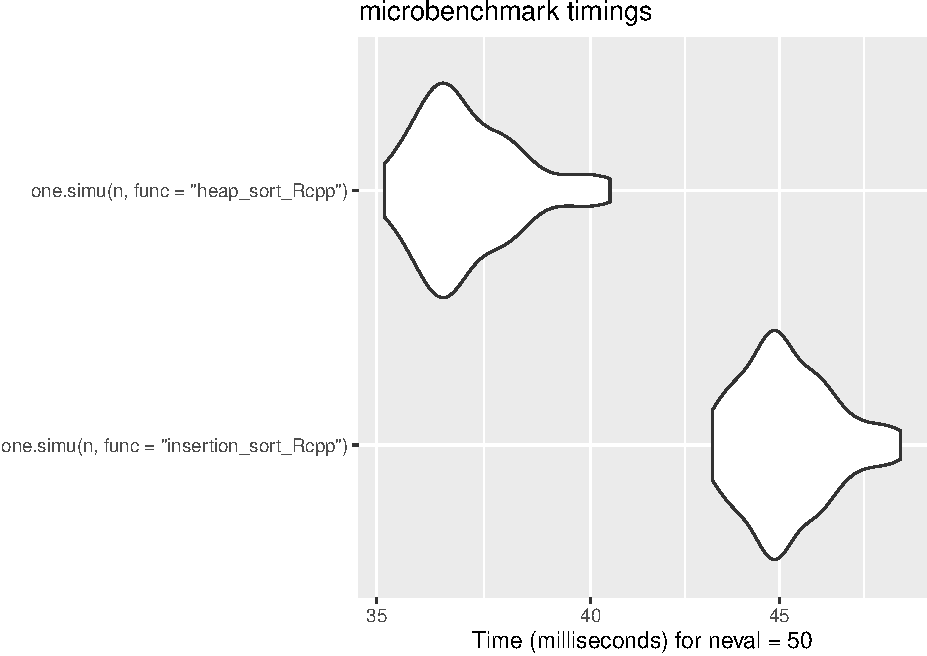
\includegraphics{Sorting_analyse_files/figure-latex/unnamed-chunk-12-1.pdf}

\begin{Shaded}
\begin{Highlighting}[]
\NormalTok{res}
\end{Highlighting}
\end{Shaded}

\begin{verbatim}
## Unit: milliseconds
##                                       expr      min       lq     mean   median
##  one.simu(n, func = "insertion_sort_Rcpp") 43.15307 44.39812 45.24246 44.95921
##       one.simu(n, func = "heap_sort_Rcpp") 35.17328 36.23912 37.06813 36.69740
##        uq      max neval
##  45.99027 48.52756    50
##  37.79249 40.49016    50
\end{verbatim}

At this data length \texttt{10000} we start having a robust difference
in running time.

\subsection{Time complexity}\label{time-complexity}

We run \texttt{nbRep\ =\ 50} times the \texttt{heap\_sort\_Rcpp}
algorithm of each value of the \texttt{vector\_n} vector of length
\texttt{nbSimus\ =\ 20}. We show the plot of the mean running time with
respect to data length.

\begin{Shaded}
\begin{Highlighting}[]
\NormalTok{nbSimus }\OtherTok{\textless{}{-}} \DecValTok{20}
\NormalTok{vector\_n }\OtherTok{\textless{}{-}} \FunctionTok{seq}\NormalTok{(}\AttributeTok{from =} \DecValTok{10000}\NormalTok{, }\AttributeTok{to =} \DecValTok{100000}\NormalTok{, }\AttributeTok{length.out =}\NormalTok{ nbSimus)}
\NormalTok{nbRep }\OtherTok{\textless{}{-}} \DecValTok{50}
\NormalTok{res\_Heap }\OtherTok{\textless{}{-}} \FunctionTok{data.frame}\NormalTok{(}\FunctionTok{matrix}\NormalTok{(}\DecValTok{0}\NormalTok{, nbSimus, nbRep }\SpecialCharTok{+} \DecValTok{1}\NormalTok{))}
\FunctionTok{colnames}\NormalTok{(res\_Heap) }\OtherTok{\textless{}{-}} \FunctionTok{c}\NormalTok{(}\StringTok{"n"}\NormalTok{, }\FunctionTok{paste0}\NormalTok{(}\StringTok{"Rep"}\NormalTok{,}\DecValTok{1}\SpecialCharTok{:}\NormalTok{nbRep))}

\NormalTok{j }\OtherTok{\textless{}{-}} \DecValTok{1}
\ControlFlowTok{for}\NormalTok{(i }\ControlFlowTok{in}\NormalTok{ vector\_n)}
\NormalTok{\{}
\NormalTok{  res\_Heap[j,] }\OtherTok{\textless{}{-}} \FunctionTok{c}\NormalTok{(i, }\FunctionTok{replicate}\NormalTok{(nbRep, }\FunctionTok{one.simu}\NormalTok{(i, }\AttributeTok{func =} \StringTok{"heap\_sort\_Rcpp"}\NormalTok{)))  }
  \CommentTok{\#print(j)}
\NormalTok{  j }\OtherTok{\textless{}{-}}\NormalTok{ j }\SpecialCharTok{+} \DecValTok{1}
\NormalTok{\}}

\NormalTok{res }\OtherTok{\textless{}{-}} \FunctionTok{rowMeans}\NormalTok{(res\_Heap[,}\SpecialCharTok{{-}}\DecValTok{1}\NormalTok{])}
\FunctionTok{plot}\NormalTok{(vector\_n, res, }\AttributeTok{type =} \StringTok{\textquotesingle{}b\textquotesingle{}}\NormalTok{, }\AttributeTok{xlab =} \StringTok{"data length"}\NormalTok{, }\AttributeTok{ylab =} \StringTok{"mean time in seconds"}\NormalTok{)}
\end{Highlighting}
\end{Shaded}

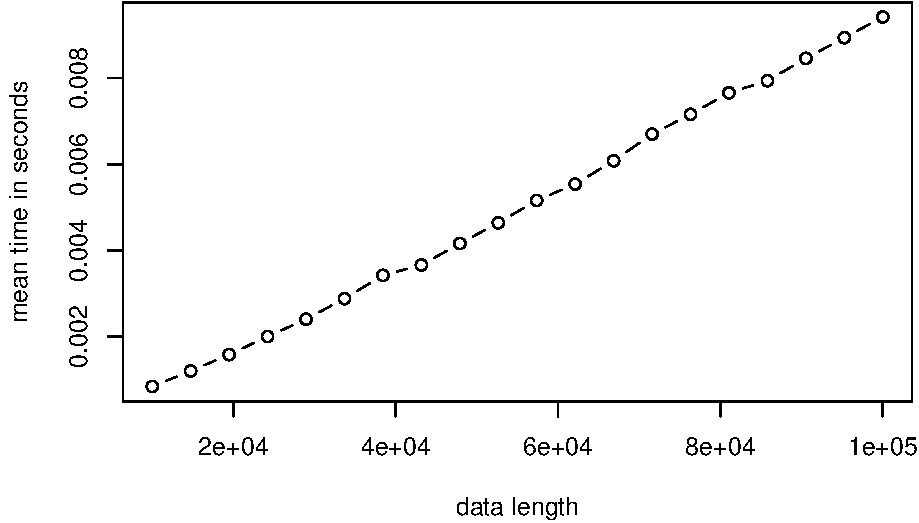
\includegraphics{Sorting_analyse_files/figure-latex/unnamed-chunk-13-1.pdf}

Same strategy but with the \texttt{insertion\_sort\_Rcpp} algorithm. We
get the power in complexity model \(O(n^r)\) by fitting a linear model
in log scale. The slope coefficient \(r\) is very close to 2 as
expected.

\begin{Shaded}
\begin{Highlighting}[]
\NormalTok{nbSimus }\OtherTok{\textless{}{-}} \DecValTok{20}
\NormalTok{vector\_n }\OtherTok{\textless{}{-}} \FunctionTok{seq}\NormalTok{(}\AttributeTok{from =} \DecValTok{5000}\NormalTok{, }\AttributeTok{to =} \DecValTok{50000}\NormalTok{, }\AttributeTok{length.out =}\NormalTok{ nbSimus)}
\NormalTok{nbRep }\OtherTok{\textless{}{-}} \DecValTok{50}
\NormalTok{res\_Insertion }\OtherTok{\textless{}{-}} \FunctionTok{data.frame}\NormalTok{(}\FunctionTok{matrix}\NormalTok{(}\DecValTok{0}\NormalTok{, nbSimus, nbRep }\SpecialCharTok{+} \DecValTok{1}\NormalTok{))}
\FunctionTok{colnames}\NormalTok{(res\_Insertion) }\OtherTok{\textless{}{-}} \FunctionTok{c}\NormalTok{(}\StringTok{"n"}\NormalTok{, }\FunctionTok{paste0}\NormalTok{(}\StringTok{"Rep"}\NormalTok{,}\DecValTok{1}\SpecialCharTok{:}\NormalTok{nbRep))}

\NormalTok{j }\OtherTok{\textless{}{-}} \DecValTok{1}
\ControlFlowTok{for}\NormalTok{(i }\ControlFlowTok{in}\NormalTok{ vector\_n)}
\NormalTok{\{}
\NormalTok{  res\_Insertion[j,] }\OtherTok{\textless{}{-}} \FunctionTok{c}\NormalTok{(i, }\FunctionTok{replicate}\NormalTok{(nbRep, }\FunctionTok{one.simu}\NormalTok{(i, }\AttributeTok{func =} \StringTok{"insertion\_sort\_Rcpp"}\NormalTok{)))  }
  \CommentTok{\#print(j)}
\NormalTok{  j }\OtherTok{\textless{}{-}}\NormalTok{ j }\SpecialCharTok{+} \DecValTok{1}
\NormalTok{\}}

\NormalTok{res }\OtherTok{\textless{}{-}} \FunctionTok{rowMeans}\NormalTok{(res\_Insertion[,}\SpecialCharTok{{-}}\DecValTok{1}\NormalTok{])}
\FunctionTok{plot}\NormalTok{(vector\_n, res, }\AttributeTok{type =} \StringTok{\textquotesingle{}b\textquotesingle{}}\NormalTok{, }\AttributeTok{xlab =} \StringTok{"data length"}\NormalTok{, }\AttributeTok{ylab =} \StringTok{"mean time in seconds"}\NormalTok{)}
\end{Highlighting}
\end{Shaded}

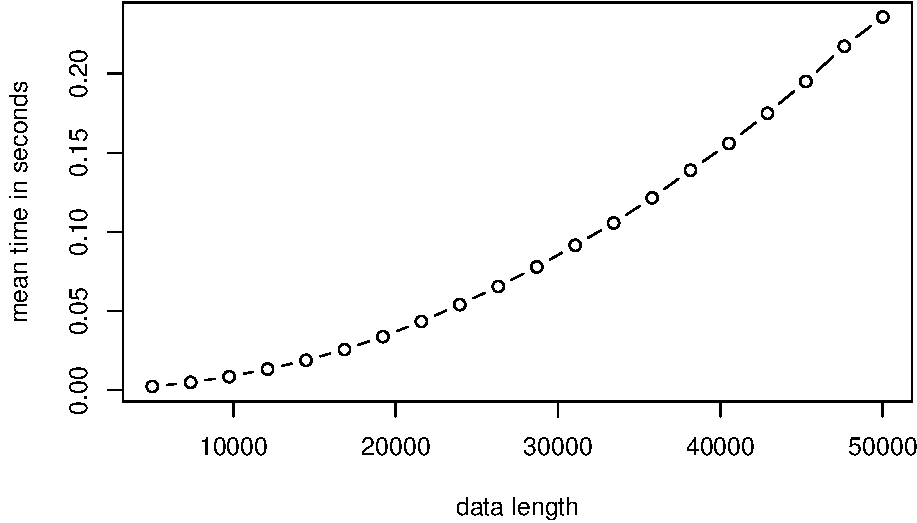
\includegraphics{Sorting_analyse_files/figure-latex/unnamed-chunk-14-1.pdf}

\begin{Shaded}
\begin{Highlighting}[]
\FunctionTok{lm}\NormalTok{(}\FunctionTok{log}\NormalTok{(res) }\SpecialCharTok{\textasciitilde{}} \FunctionTok{log}\NormalTok{(vector\_n))}
\end{Highlighting}
\end{Shaded}

\begin{verbatim}
## 
## Call:
## lm(formula = log(res) ~ log(vector_n))
## 
## Coefficients:
##   (Intercept)  log(vector_n)  
##       -23.311          2.022
\end{verbatim}

\end{document}
